% ---------------------------------------------------------------------------
% Section 3: Preregistered Protocol (slimmed: implementation/data details
% moved to Section 4 Experimental Setup per venue convention)
% ---------------------------------------------------------------------------
\section{Preregistered Protocol}\label{sec:protocol}

The protocol was preregistered (v1.0, with an append-only revision log
R1--R5 disclosed in Section~\ref{sec:limitations-revision} and the full
hash chain in Appendix~\ref{app:hashchain}) \emph{before} any
test-segment metric was computed; the confirmation-set arm list was
amended in R5 based on dev-set evidence only, with the ruling preceding
the launch of the confirmation runs and the confirmation data untouched
throughout. This section states the locked decisions; datasets,
implementation details, and the statistical protocol are specified in
Section~\ref{sec:setup}.

\subsection{Detection Interface (Teacher Lock)}\label{sec:interface}
The teacher is a frozen TSFM combined with a fixed, causal detection
pipeline: (i)~context-wise $z$-normalization using statistics of the
context window only; (ii)~one-step probabilistic forecasting of $x_t$
from $x_{<t}$, with the \emph{median} quantile taken as the point
forecast (uniform across model families); (iii)~per-channel absolute
residuals $|x_{t,c}-\hat{x}_{c}(t)|$; (iv)~cross-channel aggregation by
\emph{max}. The teacher score is therefore $s_T(t)=g(x_{\le t})$;
quantile-interval scoring is deliberately excluded (interface
sensitivity belongs to our companion audit). Context length is each
model's library default and is recorded in the cache metadata.
Distillation aligns the student to exactly this interface. The student
input window ends at the same timestamp the teacher scores, so student
and teacher scores are timestamp-aligned by construction. After
training, the teacher is removed from the deployment path entirely, and the
student is the only inference-time artifact. Input windows are
leakage-audited by arm: score-distilled students (A/C) receive the
window $x_{t-L+1..t}$ \emph{including} the current observation $x_t$,
whereas the regression arms (B1/B2) receive $x_{t-L..t-1}$ and predict
$x_t$, so the prediction target never enters the input. The teacher
scores with a 512-point context and the students with 128-point
windows; the interface ablation at $L{=}512$ (R7, exploratory, five flows)
does not support this asymmetry as the driver of the ladder conclusion
(four of five flows), though full information-set
equalization across all arms remains future work. Figure~\ref{fig:pipeline} summarizes the locked design.

\begin{figure}[t]
\centering
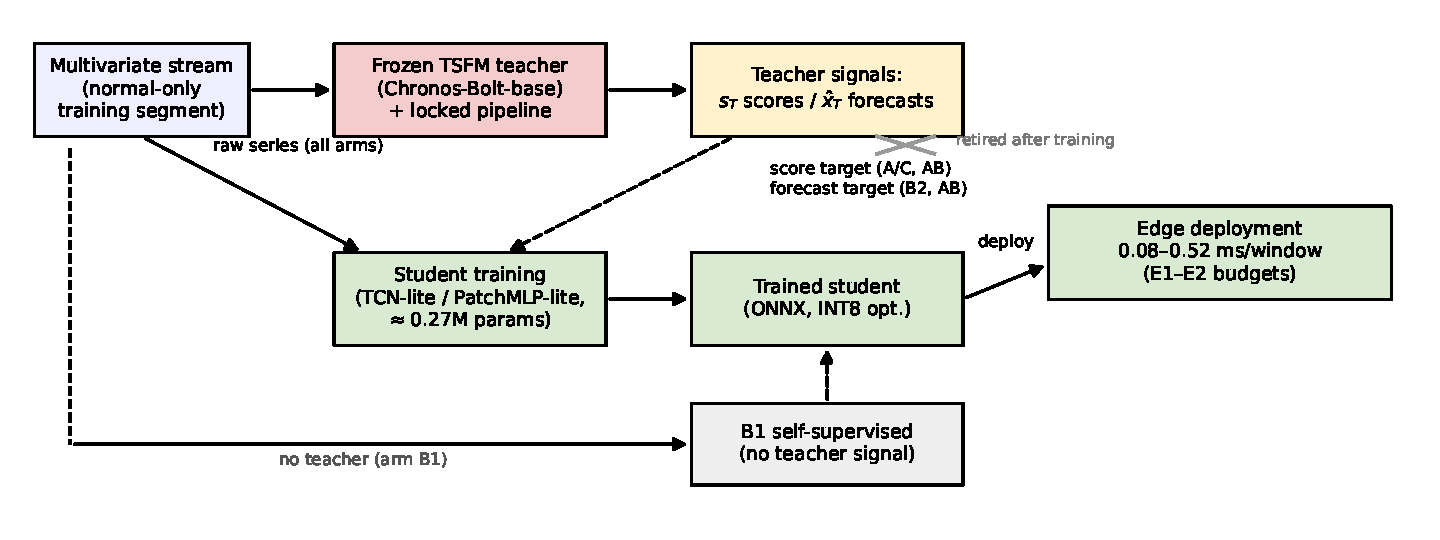
\includegraphics[width=\textwidth]{figures/fig_pipeline.pdf}
\caption{Study design. The frozen TSFM teacher (Chronos-Bolt-base behind the
locked causal scoring interface of Section~\ref{sec:interface}) provides two
candidate distillation signals to the student training stage: its anomaly
scores $s_T$ (arms A/C and the AB hybrid) and its point forecasts
$\hat{x}_T$ (arm B2 and AB). Arm B1 receives no teacher signal and trains
on the raw stream only. After training,
the teacher is retired. Only the exported student artifact (ONNX, optional
INT8) is deployed and timed.}
\label{fig:pipeline}
\end{figure}

\subsection{Three-Axis Evaluation Framework}\label{sec:axes}
All arms are evaluated on three axes. \textbf{Quality} is VUS-PR
(primary) and VUS-ROC (secondary), never using point adjustment or
thresholded $F_1$. \textbf{Fidelity} measures how faithfully the student
reproduces the teacher's scoring behavior (full-series and tail-restricted
rank agreement); it is a diagnostic axis, reported even when it conflicts
with quality. \textbf{Cost} is measured on exported inference artifacts
(ONNX, optional INT8), never on training checkpoints, under a
single-thread deployment protocol with full environment disclosure.
Formal definitions, tools, and protocols are tabulated in
Table~\ref{tab:metrics}.

\subsection{Arms and Controls}\label{sec:arms}
The preregistered arms are: the \textbf{score arm (A)}, regressing a
Huber loss to the teacher score $s_T$; the \textbf{ranking arm (C)}, a
RankNet-style objective~\cite{burges2005ranknet} over sampled within-stream pairs (relational distillation in the spirit of RKD\cite{park2019rkd}); the
\textbf{self-supervised control (B1)}, training the same backbone by
next-step regression \emph{without any teacher signal}; the
\textbf{forecast-distillation control (B2)}, regressing the teacher's
point forecast (DistilTS-style); the \textbf{hybrid (AB)}, coupling the
score objective with a $\lambda$-weighted forecast-alignment term; a
\textbf{linear floor}; and fixed references, namely the frozen teacher (T0)
and a fixed-configuration PCA-reconstruction baseline fitted on the
training segment only. Causal Matrix Profile and LOF were designated as auxiliary classical
baselines. Causal Matrix Profile was ultimately not executed (deviation
disclosed in R5): a faithful causal implementation with the full tuning
budget was judged disproportionate to its marginal value. LOF was later
added in a window-feature form under revision R11, fit on the full
unlabeled test segment (transductive, non-streaming), alongside two
zero-tuning streaming scorers. Full arm definitions, the
comparison table, and implementation details are in
Section~\ref{sec:setup-arms}.

\subsection{Preregistration and Staging}\label{sec:staging}\label{sec:limitations-revision}
The study proceeds in two source-blocked stages: an \emph{exploration} stage
on 20 development flows (arm selection, ablations, mechanism controls)
and a \emph{confirmation} stage on 9 held-out flows from source-blocked
collections (one disclosed NAB exception), at increased seed count
(3 seeds per arm on development auxiliary arms, 10 on the confirmation
stage). The preregistration was amended five
times through the append-only log (R1--R5), each before the affected
measurements and each disclosed with its trigger in the revision
history; three further revisions (R6--R8) registered exploratory
controls after the confirmation stage began, and are flagged as such in
the hash chain (Appendix~\ref{app:hashchain}). The confirmatory analyses are exactly the three preregistered
pairwise comparisons of the confirmation stage, and all other analyses
(macro rankings, conditional morphology analysis, the selection table,
and the shuffled-teacher control) are exploratory and labelled as such.
Sibling-project reuse of teacher caches is disclosed, as is the fact
that the teacher pipeline configuration is shared with a companion
audit study.
